\section{Evaluation Results of \system}
\label{sec:evaluation_of_phoenix}

In this section, we discuss the evaluation results for both the signature synthesizer
and monitor components. In order to evaluate \system as both a warning system
and defense mechanism, we evaluate these two different implementations separately.
Due to space constraints, we report the results for 5 attacks here and
the rest can be found in the Appendix.
\subsection{Signature Synthesizer Evaluation}
We evaluate our \signatureSynthesizer{}s based on the research questions discussed in Section~\ref{sec:evaluation_criteria}.

\paragraph{Effectiveness of generated signatures ($\mathsf{QS_1}$).}
For evaluating the effectiveness of the synthesized signatures,
we replay the set of testing traces to a device running \system in our testbed (set up with srsLTE~\cite{gomez2016srslte} and
USRP~\cite{usrp}), and measure precision, recall, and F1 score for
identifying those vulnerability signatures at runtime.
%

\begin{table}[]
	\centering
  %\resizebox{.8\columnwidth}{!}{

	\begin{tabular}{|c|l|l|l|l|}
		\hline
		\textbf{Attack}                         & \textbf{Monitor} & \textbf{Precision} & \textbf{Recall} & \textbf{F1} \\ \hline
		\multirow{3}{*}{AKA Bypass}             & PLTL             & 1                  & 1               & 1           \\ \cline{2-5}
		& DFA              & 1                  & 0.95            & 0.97       \\ \cline{2-5}
		& MM               & 1                  & 1               & 1           \\ \hline
		\multirow{3}{*}{IMSI Cracking}          & PLTL             & 1                  & 1               & 1           \\ \cline{2-5}
		& DFA              & 1                  & 1               & 1           \\ \cline{2-5}
		& MM               & 0.67              & 1               & 0.80       \\ \hline
		\multirow{3}{*}{Measurement Report}     & PLTL             & 1                  & 1               & 1           \\ \cline{2-5}
		& DFA              & 0.95              & 0.83           & 0.89       \\ \cline{2-5}
		& MM               & 1                  & 1               & 1           \\ \hline
		\multirow{3}{*}{Numb Attack}            & PLTL             & 1                  & 1               & 1           \\ \cline{2-5}
		& DFA              & 1                  & 1               & 1           \\ \cline{2-5}
		& MM               & 1                  & 1               & 1           \\ \hline
		\multirow{3}{*}{RLF Report}             & PLTL             & 1                  & 1               & 1           \\ \cline{2-5}
		& DFA              & 0.83              & 0.64           & 0.72       \\ \cline{2-5}
		& MM               & 1                  & 1               & 1           \\ \hline
	\end{tabular}
  %}
	\caption{Effectiveness results for all monitors with maximum data each monitor can consume (MM stands for Mealy Machine). Note that all scores are in the range 0 to 1.}
	\label{tab:effectiveness_max_data}
\end{table}

Table~\ref{tab:effectiveness_max_data} presents the precision, recall and F1 score
achieved by our \signatureSynthesizer{}s for identifying different attacks at runtime.
The signatures used in this experiment were generated with $2,500$ traces for
DFA and Mealy Machine, and up $1,250$ for PLTL due to the synthesizer
timing out. The figure
demonstrates that all of the approaches were able to identify the
existing attacks with a high degree of success.
Among the different synthesizers, DFA, however,
produced a higher number of false positives (21.5\%)
and false negatives (17.1\%) on average whereas
Mealy Machine and PLTL turn out to be more reliable;
producing a significantly less number of false
positives ($\sim\!\!$ 0.03\%) and false negatives ($\sim\!\!$ 0.01\%).

The perfect F1 score for \pltl across different attacks can be attributed
to the fact that these control-plane attacks have
a highly discernible signature, which can be seen as the temporal property
which all variants of the attacks violate. For instance,
the signature synthesized for the RLF Report Attack \cite{privacy_ndss16} is the following:
$\ueInformationRequest \Rightarrow (\neg \rrcConnectionRequest \since \securityModeComplete)$. Since this signature precisely describes the behavior of the attack, regardless of the variant,
it enables \system to detect the attack with a perfect F1 score.


Another interesting result shown in Table~\ref{tab:effectiveness_max_data}
is that Mealy Machine based monitor outperforms the DFA based one in the
majority of the cases. This is because
DFA learns only on up to 2,500 traces for an individual attack whereas
Mealy Machine learns from all the attack traces (2,500 * 15) and therefore
has more information to learn from.


\paragraph{Scalability ($\mathsf{QS_2}$).}
We primarily consider signature learning time as an effective and
indirect indicator to the scalability of the corresponding signature synthesizer.
The lower the learning time, the higher the scalability. That signifies that scalability time is inversely
proportional to the signature learning time. Therefore, to evaluate the scalability of
the three proposed signature synthesizers (DFA, MM, and PLTL),
we vary the sample size of the training sets to 50, 100, 250, 500, 1250, and 2500, and measure
the learning time required by a synthesizer for each of the attacks.
%by invoking them with the different sample sizes (50, 100, 250, 500, 1250, and 2500).
Figure~\ref{fig:learning_time} presents the results of this evaluation in which the Y-axis is seconds in the logarithmic scale and
the X-axis is the training dataset size.

Figure~\ref{fig:learning_time} shows that our \pltl signature synthesizer takes considerably more time to
synthesize a signature as compared to DFA and MM synthesizers. This large discrepancy can be attributed to the fact
that the \pltl synthesizer is a \emph{search based algorithm}. The search space
grows very quickly as the depth of the abstract syntaxt tree (AST) increases. On the other hand,
RPNI \cite{rpni} proves to scale quite well because RPNI is a polynomial time algorithm while SAT is NP-Complete.
For instance, training the AKA Bypass~\cite{kim_ltefuzz_sp19} attack with \pltl synthesizer takes a significantly higher amount
of time than others. Though \pltl synthesizer for AKA Bypass attack quickly times out,
the same synthesizer does not time out for other attacks, such as the Numb Attack~\cite{lteinspector} until it reaches
$1250$ traces. This is due to the much deeper AST for AKA Bypass \pltl signature than that for the Numb Attack.

\begin{figure}[t]
 \centering
 \resizebox{.8\columnwidth}{!}{\input{resources/lte-training-plot.tikz}}
 \caption{Time to learn DFA, PLTL and Mealy Machine.
 %\fa{Training times for each data set and size. Mealy Machine consider all attacks together.}
 }
 \label{fig:learning_time}
\end{figure}

\paragraph{Impact of training set size on signature quality ($\mathsf{QS_3}$).}
Since real-life cellular attack traces are difficult to obtain,
we aim at evaluating whether or not more training data generate a
higher quality signature. We consider a high quality signature as
one that achieves a perfect F1 score. In other words, F1 score and signature quality are proportional to each other. To
evaluate this, we vary the size of the training datasets
and measure the synthesizers' effectiveness at detecting the attacks. %Results are presented
%in Figure \ref{fig:effectiveness_vs_sample_size}.

Figure \ref{fig:effectiveness_vs_sample_size}
shows that all three signature synthesizers achieve high F1 score when
training on 500 traces, with the exception of AKA Bypass for DFA, which
goes down as more training data is given. As the RPNI learning process
is highly dependent on the exact set of input traces, this discrepancy can be
attributed to the variability of the input traces. Note that, our \pltl signature synthesizer
achieves a perfect F1 score across all attacks, regardless of the training
dataset size, because of its usage of exhaustive search to learn a
precise but highly generalizable signature.


\begin{figure}[t]
	\centering
	\resizebox{.8\columnwidth}{!}{% This file was created by tikzplotlib v0.9.1.
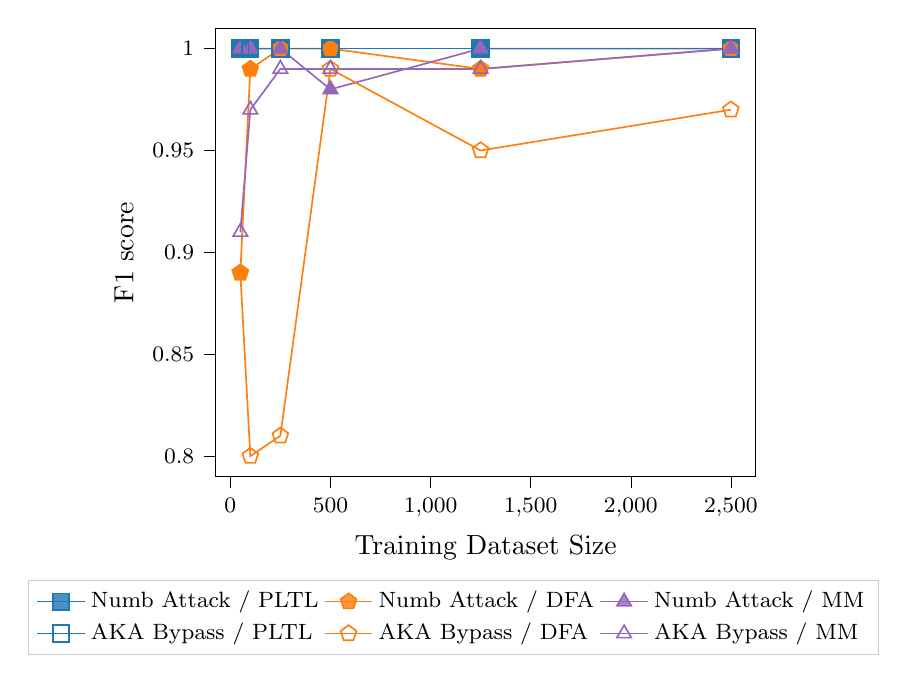
\begin{tikzpicture}

\definecolor{color0}{rgb}{0.12156862745098,0.466666666666667,0.705882352941177}
\definecolor{color1}{rgb}{1,0.498039215686275,0.0549019607843137}
\definecolor{color2}{rgb}{0.172549019607843,0.627450980392157,0.172549019607843}
\definecolor{color3}{rgb}{0.83921568627451,0.152941176470588,0.156862745098039}
\definecolor{color4}{rgb}{0.580392156862745,0.403921568627451,0.741176470588235}
\definecolor{color5}{rgb}{0.549019607843137,0.337254901960784,0.294117647058824}
\definecolor{color6}{rgb}{0.10588,0.28627,0.70980}

\begin{axis}[
legend columns = 3,
legend cell align={left},
%legend style={fill opacity=0.8, draw opacity=1, text opacity=1, at={(0.97,0.03)}, anchor=south east, draw=white!80!black},
legend style={fill opacity=0.8, draw opacity=1, text opacity=1, at={(0.44,-0.23)}, anchor=north, draw=white!80!black, font=\footnotesize},
tick align=outside,
tick pos=left,
title={},
x grid style={white!69.0196078431373!black},
xlabel={Training Dataset Size},
xmin=-72.5, xmax=2622.5,
xtick style={color=black},
y grid style={white!69.0196078431373!black},
ylabel={F1 score},
ymin=0.79, ymax=1.01,
ytick style={color=black},
tick label style={font=\footnotesize}
]
\addplot [semithick, color0, mark=square*, mark size=3, mark options={solid}]
table {%
50 1
100 1
250 1
500 1
1250 1
2500 1
};
\addlegendentry{Numb Attack / PLTL}
\addplot [semithick, color1, mark=pentagon*, mark size=3, mark options={solid}]
table {%
50 0.89
100 0.99
250 1
500 1
1250 0.99
2500 1
};
\addlegendentry{Numb Attack / DFA}
\addplot [semithick, color4, mark=triangle*, mark size=3, mark options={solid}]
table {%
50 1
100 1
250 1
500 0.98
1250 1
2500 1
};
\addlegendentry{Numb Attack / MM}
\addplot [semithick, color0, mark=square, mark size=3, mark options={solid}]
table {%
50 1
100 1
250 1
500 1
1250 1
2500 1
};
\addlegendentry{AKA Bypass / PLTL}
\addplot [semithick, color1, mark=pentagon, mark size=3, mark options={solid}]
table {%
50 0.89
100 0.8
250 0.81
500 0.99
1250 0.95
2500 0.97
};
\addlegendentry{AKA Bypass / DFA}
\addplot [semithick, color4, mark=triangle, mark size=3, mark options={solid}]
table {%
50 0.91
100 0.97
250 0.99
500 0.99
1250 0.99
2500 1
};
\addlegendentry{AKA Bypass / MM}
\end{axis}

\end{tikzpicture}
}
	\caption{Training size and effectiveness comparison.
		%\fa{Training times for each data set and size. Mealy Machine consider all attacks together.}
	}
	\label{fig:effectiveness_vs_sample_size}
\end{figure}

Since the \pltl synthesizer is able to produce a highly generalizable
signature regardless of the training dataset in the previous experiment,
we decide to analyze this further by discovering the minimum attack traces
required to generate a high quality signature. We consider a high quality signature is
one that achieves a perfect F1 score. To perform this experiment, we fix
the benign traces to $25$ and vary the number of attack traces from $1$ to $25$.
The results can be found in
Table \ref{tab:minimum_attack_traces}. These results show that the \pltl synthesizer
can rapidly produce a high quality signature. Both the RLF Report and Measurement
Report privacy attacks prove to require a larger number of attack traces.
This can be attributed to the fact that these signatures are more complex than
others, with the exception of the AKA Bypass attack, however, more variants exist.


 These results show that the \pltl
synthesizer can rapidly produce a high quality signature.
Another observation that is obvious is the fact that Measurement Report and
RLF Report require more attack traces than others. This can be attributed to a couple
of reasons. The first reason behind this result, is that these two attacks require a
larger search space since the alphabet is bigger than the others. The second
reason is that these attacks are more complex than others, with the exception
of the AKA Bypass attack which can be seen as a stepping stone for both. In addition,
these results can also attributed to the fact that our \pltl synthesizer blindly
searches for solutions instead of using the given traces to narrow down the search
space.

\begin{table}[]
  \centering
  %\resizebox{.8\columnwidth}{!}{

\begin{tabular}{|c|c|c|}
\hline
\textbf{Attack} & \textbf{Minimum Attack Trace} & \textbf{\# of Variations} \\ \hline
AKA Bypass & 3 & 2 \\ \hline
IMSI Cracking & 1 & 1 \\ \hline
Measurement Report & 11 & 5 \\ \hline
RLF Report & 8 & 2 \\ \hline
Numb Attack & 3 & 2 \\ \hline
\end{tabular}
%}
\caption{Minimum attack traces (and variations), required to generate a high quality signature (Perfect F1 score) using PLTL synthesizer.}
\label{tab:minimum_attack_traces}
\end{table}




\paragraph{Signature Synthesizer Evaluation Conclusion.}
%In this subsection, we evaluated the proposed signature synthesizers and
%compared them using metrics.
The \pltl synthesizer proved to not scale as well
as RPNI \cite{rpni} based approaches, however, it proved to quickly generated
highly generalizable signature. In fact, such a signature generation with a minimal number of traces is
critical since generating attack traces is a challenging task for cellular networks.
Therefore, we conclude that the \pltl synthesizer outperforms
the RPNI \cite{rpni} approaches.





\subsection{Monitor Evaluation (Warning System)}
\label{sec:monitor_evaluation_warning_system}
In this subsection, we answer the research questions driving the evaluation
of three different monitoring approaches (i.e., \pltl, DFA, and Mealy Machine)
when considering a warning system instantiation.

\paragraph{Efficiency ($\mathsf{QWS_1}$).}
One of the key factors in identifying the best monitor instantiation
is the number of messages each monitor can process per second.
For this, we perform a stress test by mimicking the modem through the
replaying of real traces captured
from MobileInsight's database \cite{mobile_insight} without any delay
between subsequent messages. We measure how long each monitor takes
to process and check for the presence of an attack by consulting
its entire signature database. Table \ref{tab:message_per_second_overall}
summarizes the processing speed (messages/second) of different
devices for different monitoring approaches running in two different layers
(RRC and NAS). In addition to this, we computed the CPU cycles required per call
to the monitor component for each device which can be found in Table \ref{tab:cpu_cycles_tab}.


\begin{table}[]
  \centering
	\begin{tabular}{|l|c|l|l|}
	\hline
	\multicolumn{1}{|c|}{\textbf{Layer}} & \textbf{Monitor} & \multicolumn{1}{c|}{\textbf{Device}} & \multicolumn{1}{c|}{\textbf{Avg. CPU Cycles}} \\ \hline
	\multirow{9}{*}{RRC} & \multirow{3}{*}{DFA} & Pixel 3 & 54,127.20 \\ \cline{3-4}
	 &  & Nexus 6P & 97,168.98 \\ \cline{3-4}
	 &  & Nexus 6 & 325,579.71 \\ \cline{2-4}
	 & \multirow{3}{*}{PLTL} & Pixel 3 & 384,282.80 \\ \cline{3-4}
	 &  & Nexus 6P & 560,255.48 \\ \cline{3-4}
	 &  & Nexus 6 & 4,065,040.65 \\ \cline{2-4}
	 & \multirow{3}{*}{MM} & Pixel 3 & 7,177.05 \\ \cline{3-4}
	 &  & Nexus 6P & 15,900.18 \\ \cline{3-4}
	 &  & Nexus 6 & 78,850.07 \\ \hline
	\multirow{9}{*}{NAS} & \multirow{3}{*}{DFA} & Pixel 3 & 81,957.62 \\ \cline{3-4}
	 &  & Nexus 6P & 136,431.23 \\ \cline{3-4}
	 &  & Nexus 6 & 599,973.33 \\ \cline{2-4}
	 & \multirow{3}{*}{PLTL} & Pixel 3 & 742,528.31 \\ \cline{3-4}
	 &  & Nexus 6P & 1,094,331.36 \\ \cline{3-4}
	 &  & Nexus 6 & 4,456,180.89 \\ \cline{2-4}
	 & \multirow{3}{*}{MM} & Pixel 3 & 7,586.85 \\ \cline{3-4}
	 &  & Nexus 6P & 14,812.58 \\ \cline{3-4}
	 &  & Nexus 6 & 78,853.99 \\ \hline
	\end{tabular}
\caption{CPU Cycles required per call to the monitor. The clock speed for the devices
are the following: Pixel 3 = 2.8 Ghz, Nexus 6P = 2.0 Ghz, and  Nexus 6 = 2.7 Ghz.}
\label{tab:cpu_cycles_tab}
\end{table}

As shown in Table \ref{tab:message_per_second_overall}, across all three
devices, Mealy Machine can process multiple orders of magnitude higher messages
per second than the other two monitoring approaches. This can be attributed to the
fact that Mealy Machine keeps only
a single internal state per layer, as compared to 10 internal states for
NAS and 5 for RRC. Moreover, Mealy Machine relies on a single dictionary
lookup to decide on the transition and whether to flag a trace as an attack.
Similar to Mealy Machine, DFA can also process messages at a much faster
rate than \pltl. This is because the DFA also relies on a simple
dictionary lookup similar to Mealy Machine for a single signature.
On the other hand, \pltl requires the evaluation of logical and
temporal operators to classify the incoming traces which is a
more expensive operation.


To put our results in perspective, we compare it with real traces.
% To compare the results of the stress test with real traces,
We compute the mean, median, standard deviation, and
maximum number of messages of real NAS and RRC traces obtained from the
MobileInsight database \cite{mobile_insight}.
We observe that on average, there were 0.02 messages per second
for NAS traffic (median=0.011, standard deviation=0.069, maximum=0.8),
and 0.2 messages per second (median=0.122, standard deviation=0.273, maximum=2.76)
for RRC traffic.

In summary,
our slowest monitor (i.e., \pltl) can handle substantially more message
per second than the NAS and RRC traffic we observed in real traces.

\begin{table}[h!]
  \centering
  %\resizebox{.8\columnwidth}{!}{

  \begin{tabular}{|c|c|l|l|l|}
  \hline
  \textbf{Layer} & \textbf{Monitor} & \textbf{Device} & \multicolumn{1}{c|}{\textbf{Avg.}} & \multicolumn{1}{c|}{\textbf{SD}} \\ \hline
  \multirow{9}{*}{RRC} & \multirow{3}{*}{DFA} & Pixel 3 & 51730.6 & 158596.4 \\ \cline{3-5}
   &  & Nexus 6P & 20582.7 & 73663.6 \\ \cline{3-5}
   &  & Nexus 6 & 8292.9 & 8636.4 \\ \cline{2-5}
   & \multirow{3}{*}{PLTL} & Pixel 3 & 7286.3 & 55599.5 \\ \cline{3-5}
   &  & Nexus 6P & 3569.8 & 12976.3 \\ \cline{3-5}
   &  & Nexus 6 & 664.2 & 58.0 \\ \cline{2-5}
   & \multirow{3}{*}{MM} & Pixel 3 & 390132.6 & 790596.7 \\ \cline{3-5}
   &  & Nexus 6P & 125784.7 & 359847.7 \\ \cline{3-5}
   &  & Nexus 6 & 34242.2 & 14377.8 \\ \hline
  \multirow{9}{*}{NAS} & \multirow{3}{*}{DFA} & Pixel 3 & 34164.0 & 224904.7 \\ \cline{3-5}
   &  & Nexus 6P & 14659.4 & 110780.6 \\ \cline{3-5}
   &  & Nexus 6 & 4500.2 & 4170.7 \\ \cline{2-5}
   & \multirow{3}{*}{PLTL} & Pixel 3 & 3770.9 & 62512.7 \\ \cline{3-5}
   &  & Nexus 6P & 1827.6 & 22226.2 \\ \cline{3-5}
   &  & Nexus 6 & 605.9 & 1472.4 \\ \cline{2-5}
   & \multirow{3}{*}{MM} & Pixel 3 & 369059.5 & 723754.8 \\ \cline{3-5}
   &  & Nexus 6P & 135020.4 & 371327.7 \\ \cline{3-5}
   &  & Nexus 6 & 34240.5 & 20397.0 \\ \hline
  \end{tabular}
  %}
\caption{Measurement of how many messages per second can each monitor classify on different devices and layers.}
\label{tab:message_per_second_overall}
\end{table}

\paragraph{Energy Consumption ($\mathsf{QWS_2}$).}
To understand the energy consumption induced by each monitor component, we
measure the battery consumption induced by \system. We perform this
experiment by connecting
the Nexus 6 to a Monsoon Meter \cite{monsoon}. The Nexus 6, unlike the other
two devices, has a removable back which makes it easier to connect to the power
meter. In this experiment, the traffic is simulated to avoid the noise induced
by the cellular connection. In addition to the radio, we switch off the screen,
Bluetooth, and Wi-Fi. We then invoke each monitor with $10k$
messages to evaluate the average power consumption. Figure \ref{fig:power_consumption_simulator}
presents the average power consumption by three different monitors along with the case when no monitor is active.
The results match the trend with that of synthesizers' effectiveness,
except for the fact that Mealy Machine consumed slightly  more electricity than
\pltl and DFA, respectively. %This is surprising since Mealy Machine performed better in the
%efficiency experiment.
This discrepancy could be attributed to
the fact that even though we disabled many power hungry components of the Android system, we
have no control as to what other applications in the device are doing. Overall
though, all monitors add negligible overhead.


\begin{figure}[t]
  \centering
	\includegraphics[width=.8\columnwidth]{figures/power_measurement_simulator.pdf}
	\caption{Power consumption on simulator in milliwatts (mW).}
	\label{fig:power_consumption_simulator}
\end{figure}

% \says{rafi}{Need to cut it short. Report and explain only the numbers. Don't need to explain how we computed that numbers.}

\paragraph{Real World Evaluation ($\mathsf{QWS_3}$).}
Vulnerability detection systems must balance false warnings with effectiveness.
If the user is bombarded with false warnings, the user would disable the
system in order to prevent continuously erroneous warnings. In light of this,
we aim to uncover how many warnings each different monitor produces
and the type of them. To carry out this experiment, we deploy \system
on two Pixel 3 devices running on four major U.S. cellular network carriers
on two different geographical areas.
In this experiment, we run \system for approximately 12 hours and use the
Pixel 3 as our daily devices, which includes driving approximately ~10 miles.
The results are shown in Table \ref{tab:real_world_warnings}. As expected by
previous results, DFA proves to be inadequate and produces a larger
amount of false warnings. We inspect each warning and uncover that the DFA
signature does not take into consideration the behavior seen by
these real networks. On the other hand, Mealy Machine produces no false warnings
and therefore would not bombard the user with these. Notably,
\pltl produces one warning on three different providers, specifically the
warning that is triggered when the EMM Information message is sent in plaintext.
After manual inspection, we discover that these in fact are not false warnings,
but misconfigurations by these three providers.


\begin{table}[]
  \centering
  \begin{tabular}{|c||*{4}{c|}}\hline
  \backslashbox{\textbf{Monitor}}{\textbf{Carrier}}
  &\textbf{US-1}&\textbf{US-2}
  &\textbf{US-3}&\textbf{US-4}\\\hline\hline
  DFA &6\xmark&7\xmark&4\xmark&4\xmark\\\hline
  PLTL &0&1\checkmark&1\checkmark&1\checkmark\\\hline
  MM &0&0&0&0\\\hline
  \end{tabular}
\caption{Number of warnings triggered by different monitor implementations in real networks
(\checkmark = Real Warnings, \xmark = False Warnings).}
\label{tab:real_world_warnings}
\end{table}

\paragraph{Evaluation Summary of Warning System Instantiation.}
%In this subsection we evaluated different monitor components and compared
%them with different metrics.
Mealy Machine proved to be highly efficient, however,
all three monitors were able to parse a significantly high number of messages per second to not
induce any delay at runtime. We then measured power consumption and
discovered that all three monitors are highly efficient by imposing a negligible
overhead. We then carried
out a real world evaluation of \system by deploying it on cellular devices with
real SIM cards and uncover that \pltl and Mealy Machine produce no false warnings,
and in fact, \pltl uncovers real misconfigurations in three of the major U.S. cellular
network carriers. In summary,
\pltl proved to be the monitor component that best satisfies the core
requirements.

\subsection{Monitor Evaluation (Defense Mechanism)}
Understanding the requirements of \system when implemented in the baseband
is crucial in order to understand its deployability. Due to this,
this subsection answers the research questions driving the evaluation of the
baseband instantiation of \system. We perform these experiments on the baseband
implementation as discussed in Section \ref{sec:baseband_implementation}.
Due to the fact that \pltl is the monitor that performed the best as shown
previously (in Section \ref{sec:monitor_evaluation_warning_system}), we focus
on the \pltl monitor.

\paragraph{Memory overhead in baseband ($\mathsf{QBB_1}$).}
Low memory overhead is critical in order for a defense mechanism to be
feasible. To analyze this overhead, we measure the
memory using the \textbf{time} Linux command capable of extracting the maximum
resident set size. We then compare the implementation
of \system in srUE (dubbed $srsUE_{PHOENIX}$) and the vanilla version of srsUE
(dubbed $srsUE_{vanilla}$). To perform this experiment, we connect the srsUE
implementations 100 times to the eNodeB and EPC by running the corresponding
components of srsLTE \cite{gomez2016srslte} on a secondary machine.

Figure
\ref{fig:baseband_implementation_memory} shows the distribution of both srsUE
implementations. The
distribution is similar in both implementations. The mean difference is only
159.25 KB.
% and at most, produces 1000 kbytes more than mean memory
% consumption of $srsUE_{vanilla}$.
To
put this result in perspective, $srsUE_{vanilla}$ on average consumes approximately
370MB, therefore, \system induces only a mere $0.04\%$ overhead.
Overall, we demonstrate that memory overhead of \system is not a major concern
in its baseband instantiation.

% can see that the memory overhead is minimum when compared to
% the memory requirements of the baseband processor itself.

\begin{figure}[t]
 \centering
 \resizebox{.8\columnwidth}{!}{\input{resources/memory_overhead_tikz_graph.tikz}}
 \caption{Probability density function for the maximum resident size (kilobytes) for \system implementation in srsUE\cite{gomez2016srslte} and vanilla srsUE.}
 \label{fig:baseband_implementation_memory}
\end{figure}
%

\paragraph{Computational overhead in baseband ($\mathsf{QBB_2}$).}
Another key point that must be analyzed is the computational overhead imposed by
\system in a baseband implementation. This is because %due to the fact that
any substantial
delay imposed by \system could affect the quality of service and result in a disruption
of service. In this experiment, we run the baseband implementation of \system running
all the monitors and measuring the time it takes for all monitors to run sequentially
by measuring the system time in microseconds with the \textbf{getrusage} c++ function.
We carried out this experiment connecting the modified version of srsUE 100 times
to an eNodeB and EPC running on a secondary machine. On average, calling all
15 monitors sequentially added an overhead of $5.43$ microseconds, with a
standard deviation of $10.8$. Overall, this experiment verifies that the overhead
induced by \system is negligible, and would unlikely to induce any
QoS or service disruption issues.
% due to its highly efficient implementation which uses
% synthesized functions to serve as the monitors.

\paragraph{Evaluation Summary of Baseband Implementation.}
%In this subsection we evaluated different monitor components and compared
%them with different metrics.
We evaluated the overhead induced by the baseband
implementation of \system in srsUE to serve as a proxy to understand the
real world requirements. \system showed to require minimal memory ($159.25$ kbytes)
and computational overhead ($5.4$ microseconds) which shows that \system could be deployed in a real baseband
implementation.
